PayPal fungiert in einer Onlinetransaktion als Zwischenhändler. Hierbei muss der Kunde aber bereits ein eingerichtetes und verlinktes Konto haben. Um sich bei PayPal zu registrieren muss man seinen Namen, seine E-Mail und eine Bankverbindung hinterlegen. Darauf wird einige Tage später ein kleiner Centbetrag überwiesen, zusammen mit einen Zahlencode, den man nur noch auf der Website eingeben muss, worauf das Konto freigeschaltet ist. Bei einer Kreditkarte ist es ein ähnliches Prozedere, wobei einige Cents abgebucht werden, bei beiden Methoden wird der Betrag ausgeglichen. Bei einem Kauf muss man vor dem Abschluss noch seine Daten seines Kontos, alias E-Mail und Passwort, was man nach eingeben des Zahlencodes einstellen kann, eintragen, diese werden dann von PayPal geprüft und der Kauf abgeschlossen. Dabei wird nicht einfach das Geld vom Konto des Käufers auf das Konto des Verkäufers gesendet. PayPal überweist das Geld direkt an das Konto des Händlers stellt aber erst Tage später per Lastschrift die Rechnung an den Käufer. Damit garantiert PayPal die schnellstmögliche Lieferung. Bei einer Rücksendung funktioniert PayPal ähnlich. Dabei wird das Geld direkt auf den PayPal-Konto gutgeschrieben, darauf ist es möglich sich auch das Geld auf sein Bankkonto überweisen zu lassen \cite{schulz}. Auch ist es möglich Geld zu transferieren, wenn es um keinen Kauf bzw. keinen Kauf auf einer Internetseite mit PayPal geht. Durch die PayPal App wurde auch das Senden vereinfacht speziell an Nahestehende, wie Freunde und Familie. Auch hat PayPal eine Funktion namens Moneypool. Hierbei handelt es sich um eine Art extra Konto, dass für einen einzigen Zweck eingerichtet worden ist. Darauf können ausgesuchte Personen, vom Ersteller voreingestellt, zugriff haben, dabei können sie aber nur Geld zum „Pool“ hinzufügen, daher auch der Name. Dadurch können beispielsweise Geschenke oder Überraschungen finanziert werden, egal ob es sich um Familienmitglieder handelt oder Arbeitskollegen, solange jeder als Freund registriert ist vom Ersteller des Moneypools \cite{PayPal}. PayPals Ziel war es Bezahlen online sicherer zu machen. Dabei stehen drei Punkte im Vordergrund: Käuferschutz, Datensicherheit, Transaktionssicherheit. Beim Käuferschutz handelt es sich um eine Regelung wobei, wenn die Beschreibung eines Artikels inakkurat ist oder der Artikel gar nicht erst ankommt, dann die volle Summe samt Porto-Gebühren auf das Konto des Käufers zurücküberwiesen wird. Die Datensicherheit ist der Vorteil, dass man seine Bankdaten nicht mit dem ganzen Internet teilen muss, sondern nur mit PayPal die alle kommenden Geschäfte für einen Abwickeln. Ebenfalls ist jede Transaktion und E-Mail von PayPal verschlüsselt wodurch die Transaktionen so sicher wie möglich versucht gestaltet zu werden. All dies hat seine Kosten, zumindest für Händler. Jegliche Transaktion von Privatpersonen sind kostenlos, solang sie im selben Land registriert sind und keine Währungsumrechnung notwendig ist. Hingegen gelten für Händler Raten, worin sie nach höheren Transaktionsvolumen höhere Gebühren zahlen müssen.

\begin{figure}[h]
    \begin{center}
        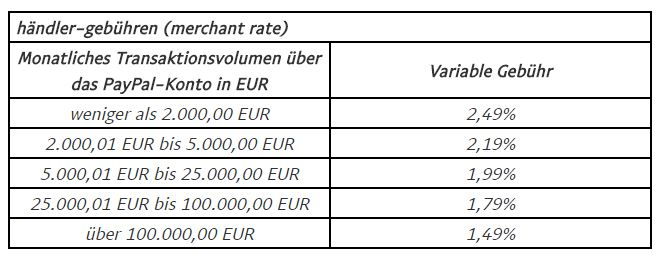
\includegraphics[width=8cm]{media/paypal.png}
        \caption{Paypal's Gebühren}
        \label{gebühren-paypal}
        \bildquelle Paypal erhöht Gebühren für Händler. In: Sellercamp (2019). https://bit.ly/3nWdMna. – aufgerufen am 22. 12. 2020
    \end{center}
\end{figure}

\noindent PayPal versucht eine Alternative zu herkömmlichen Bezahlungsmethoden zu sein, obwohl die Sicherheit und der Service von PayPal auch von anderen Unternehmen geleistet werden kann.
